\documentclass[11pt]{article}
\usepackage[nocap]{ctex}
\usepackage{algorithm}
\usepackage{algorithmic}
\usepackage{amsmath}
\usepackage{titletoc}
\floatname{algorithm}

\usepackage{geometry}
\geometry{left=2.0cm, right=2.0cm, top=2.5cm, bottom=2.5cm}

\usepackage{graphicx}
\usepackage{pdfpages}
%%%%%%%%%%%%% C++ Code
\usepackage{color}
\usepackage{xcolor}
\definecolor{keywordcolor}{rgb}{0.8,0.1,0.5}
\usepackage{listings}
\lstset{breaklines}%这条命令可以让LaTeX自动将长的代码行换行排版
\lstset{extendedchars=false}%这一条命令可以解决代码跨页时,章节标题,页眉等汉字不显示的问题
\lstset{language=C++, %用于设置语言为C++
	keywordstyle=\color{keywordcolor} \bfseries, 
	identifierstyle=,
	basicstyle=\ttfamily, 
	commentstyle=\color{blue} \textit,
	stringstyle=\ttfamily, 
	showstringspaces=false,
	%frame=shadowbox, %边框
	captionpos=b
}
%%%%%%%%%%%%% C++ Code





\title{Metis \\ for Algorithm Design and Analysis}
\author{Aha Group}
\date{Oct 8, 2016}

\begin{document}
\begin{titlepage}

\newcommand{\HRule}{\rule{\linewidth}{0.5mm}}
\center
\textsc{\LARGE Templates}\\[1.5cm] 
\textsc{\Large Shanghai Jiaotong University}\\[0.5cm]
%\textsc{\large ACM Class}\\[0.5cm]
\HRule \\[0.4cm]
{ \huge \bfseries Metis}\\[0.4cm] 
\HRule \\[1.5cm]

\begin{minipage}{0.4\textwidth}
\begin{flushleft} \large
\emph{Member:}\\
 \textsc{Sishan Long \\ Yutong Xie \\ Jingyi Cai}
\end{flushleft}
\end{minipage}
~
\begin{minipage}{0.4\textwidth}
\begin{flushright} \large
\emph{Coach:} \\
\textsc{Yunqi Li \\ Xueyuan Zhao}
\end{flushright}
\end{minipage}\\[4cm]


%{\large \today}\\[3cm] 
%\includegraphics{frontpage.jpeg}

\vfill

\end{titlepage}
	\newpage	
	
	\tableofcontents
	\newpage
	
	\section{数学}
		\subsection{FFT}
		\lstinputlisting{FFT_xxxxxyt.cpp}
		\subsection{NTT}
		\lstinputlisting{NTT.cpp}
		\subsection{高斯消元}
		\lstinputlisting{高斯消元算行列式.cpp}
		\subsection{中国剩余定理}
		\lstinputlisting{中国剩余定理.cpp}
		\subsection{Polya寻找等价类}
		\lstinputlisting{Polya寻找等价类.cpp}
		\subsection{拉格朗日插值}
		\includegraphics{拉格朗日插值1.jpg}\\
		\includegraphics{拉格朗日插值2.jpg} 
		\subsection{欧拉公式}
		\lstinputlisting{欧拉公式.cpp}
		\subsection{求行列式的值}
			行列式有很多性质,第$a$行$*k$加到第$b$行上去,行列式的值不变。\\
			三角行列式的值等于对角线元素之积。\\
			第$a$行与第$b$行互换,行列式的值取反。\\
			常数*行列式,可以把常数乘到某一行里去。\\
			注意:全是整数并取模的话当然需要求逆元
		\subsection{莫比乌斯}
		$$\sum_{d|n}\mu(d)=[n==1]$$ 
		$$ \mu(m)=\left\{
		\begin{array}{rcl}
		(-1)^r      &      & {m=p_1p_2...p_r}\\
		0  &      & {p^2|n}
		\end{array} \right.
		$$
		某个Mobius推倒:\\
		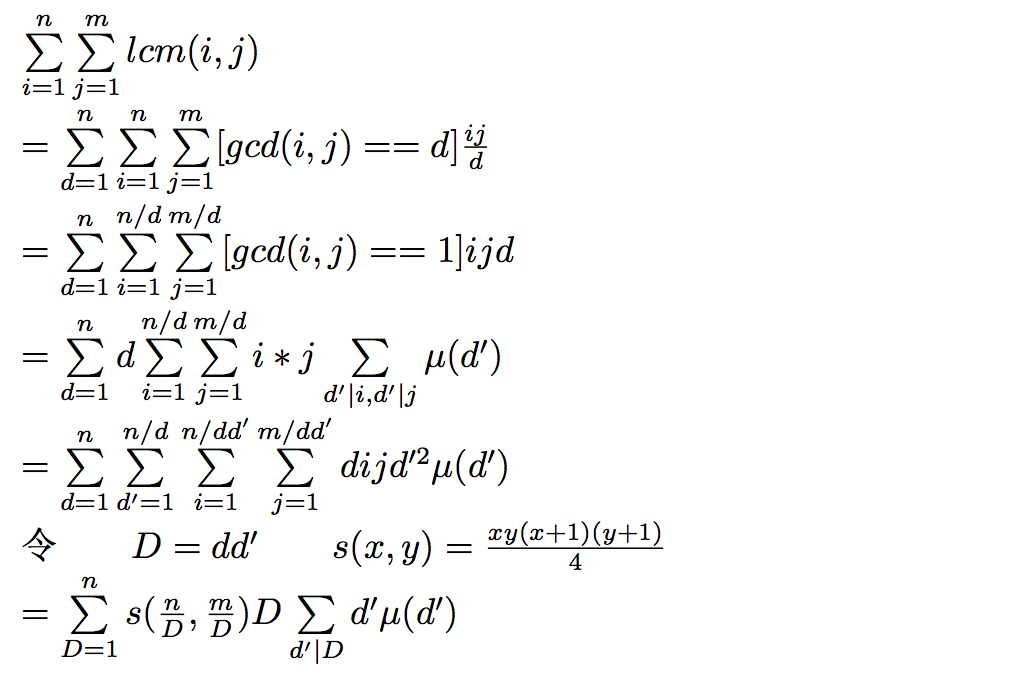
\includegraphics{Mobius.png}
		$$\mu(n) = \begin{cases}
	1 & \text{若}n=1\\
	(-1)^k & \text{若}n\text{无平方数因子,且}n = p_1p_2\dots p_k\\
	0 & \text{若}n\text{有大于}1\text{的平方数因数}
\end{cases}$$
$$\sum_{d|n}{\mu(d)} = \begin{cases}
	1 & \text{若}n=1\\
	0 & \text{其他情况}
\end{cases}$$
$$g(n) = \sum_{d|n}{f(d)} \Leftrightarrow f(n) = \sum_{d|n}{\mu(d)g(\frac{n}{d})}
,       g(x) = \sum_{n=1}^{[x]}f(\frac{x}{n}) \Leftrightarrow f(x) = \sum_{n=1}^{[x]}{\mu(n)g(\frac{x}{n})}$$

		\subsection{Cayley公式与森林计数}
		Cayley公式是说,一个完全图$K_n$有$n^{n-2}$棵生成树,换句话说$n$个节点的带标号的无根树有$n^{n-2}$个。

令$g[i]$表示点数为$i$的森林个数,$f[i]$表示点数为$i$的生成树计数$(f[i]=i^{i-2})$
那么便有$$g[i]=\sum (g[i-j] \times cnr[i-1][j-1] \times f[j])$$
$$g[i]=\sum \frac{g[i-j] \times fac[i-1] \times f[j]}{fac[j-1] \times fac[i-j]}=fac[i-1] \times \sum (\frac{f[j]}{fac[j-1]} \times \frac{g[i-j]}{fac[i-j]})$$
	
	\section{数据结构}
		\subsection{KD Tree}
		\lstinputlisting{KD-tree.cpp}
		\subsection{Splay by xyt}
		\lstinputlisting{Splay_xxxxxyt.cpp}
		\subsection{主席树 by cjy}
		\lstinputlisting{主席树_cjy.cpp}
		\subsection{主席树 by xyt}
		\lstinputlisting{主席树_xxxxxyt.cpp}
		\subsection{树分治 by xyt}
		\lstinputlisting{树分治_xxxxxyt.cpp}
		\subsection{树链剖分 by cjy}
		\lstinputlisting{树链剖分_cjy.cpp}
		\subsection{树链剖分 by xyt}
		\lstinputlisting{树链剖分_xxxxxyt.cpp}
		\subsection{点分治 by xyt}
		\lstinputlisting{点分治_xxxxxyt.cpp}
		\subsection{LCT by xyt}
		\lstinputlisting{LCT_xxxxxyt.cpp}
	\section{计算几何}
		\subsection{向量旋转}
		\lstinputlisting{向量旋转.cpp}
		\subsection{至少被i个圆覆盖的面积}
		时间复杂度: $n^2logn$
		\lstinputlisting{圆的面积.cpp}
		\subsection{计算几何杂}
		\lstinputlisting{计算几何杂.cpp}
		\subsection{三维变换}
		\lstinputlisting{三维变换.cpp}
	\section{字符串}
		\subsection{AC-Automachine by cjy}
		\lstinputlisting{AC-Automachine_cjy.cpp}
		\subsection{AC-Automachine by xyt}
		\lstinputlisting{AC-Automachine_xxxxxyt.cpp}
		\subsection{后缀数组}
		\lstinputlisting{后缀数组.cpp}
		\subsection{扩展KMP}
		\lstinputlisting{扩展KMP.cpp}
		\subsection{回文树}
		\lstinputlisting{回文树.cpp}
		\subsection{SAM by lss}
		\lstinputlisting{SAM_lss.cpp}
		\subsection{SAM by xyt}
		\lstinputlisting{SAM_xxxxxyt.cpp}
	\section{图论}
		\subsection{图论相关}
		
		1. 差分约束系统\\
  (1)以 x[i] - x[j] <= c 为约束条件,j -> i : c,求最短路得到的是 x[i] <= x[s] 的最大解,存在负权回路无解\\
  (2)以 x[i] - x[j] >= c 为约束条件,j -> i : c,求最长路得到的时 x[i] >= x[s] 的最小解,存在正权回路无解
  // 若有 x[i] = x[j] 则 i <-0-> j\\
2. 最大闭合权子图\\
  s 向正权点连边,负权点向 t 连边,边权为点权绝对值,再按原图连边,边权为INF\\
3. 最大密度子图:max{$\frac{|E'|}{|V'|}$}\\
  (1)猜测答案 g 若最大流大于 EPS 则 g 合法\\
  (2)s -> v: INF, u -> t : INF + g - deg[u], u -> v : 1.00\\
4. 2-SAT\\
  利用对称性建图,若 u 与 u' 在同一强连通分量中,则无解,若有解输出方案,拓扑排序后自底向上(从 ind = 0 到 otd = 0)选择删除\\
5. 最小割\\
  (1)二分图最小点权覆盖集:s -> u : w[u], u -> v : INF, v -> t : w[v]\\
		\subsection{SteinerTree by cjy}
		\lstinputlisting{SteinerTree_cjy.cpp}
		\subsection{LCA by xyt}
		\lstinputlisting{LCA_xxxxxyt.cpp}
		\subsection{KM}
		\lstinputlisting{KM.cpp}
		\subsection{KM三次方}
		\lstinputlisting{KM-N^3.cpp}
		\subsection{Dinic by cjy}
		\lstinputlisting{Dinic_cjy.cpp}
		\subsection{网络流 by xyt}
		\lstinputlisting{网络流_xxxxxyt.cpp}
		\subsection{最大密度子图}
		\lstinputlisting{最大密度子图.cpp}
		\subsection{强联通分量}
		\lstinputlisting{强联通分量.cpp}
		\subsection{边双联通分量}
		\lstinputlisting{边双联通分量.cpp}
		\subsection{点双联通分量加构造森林块}
		\lstinputlisting{点双联通分量加构造森林块.cpp}
		\subsection{K短路}
		\lstinputlisting{k短路.cpp}
	\section{其他}
		\subsection{Dancing Links(精确覆盖及重复覆盖)}
		\lstinputlisting{DancingLinksX_xxxxxyt.cpp}
		\subsection{序列莫队}
		\lstinputlisting{序列莫队_xxxxxyt.cpp}
		\subsection{模拟退火}
		\lstinputlisting{模拟退火.cpp}
		\subsection{Java}
		\lstinputlisting{Main.java}
		\subsection{博弈论相关}
		\begin{enumerate}
	\item Anti-SG:
		规则与Nim基本相同,取最后一个的输。
		先手必胜当且仅当:
		(1) 所有堆的石子数都为1且游戏的SG值为0;
		(2) 有些堆的石子数大于1且游戏的SG值不为0。
	\item SJ定理:
		对于任意一个Anti-SG游戏,如果我们规定当局面中,所有的单一游戏的SG值为0 时,游戏结束,则先手必胜当且仅当:
		(1) 游戏的SG函数不为0且游戏中某个单一游戏的SG函数大于1;
		(2) 游戏的SG函数为0且游戏中没有单一游戏的SG函数大于1。
	\item Multi-SG游戏:
		可以将一堆石子分成多堆.
	\item Every-SG游戏:
		每一个可以移动的棋子都要移动.
		对于我们可以赢的单一游戏,我们一定要拿到这一场游戏的胜利.
		只需要考虑如何让我们必胜的游戏尽可能长的玩下去,对手相反。
		于是就来一个DP,
		step[v] = 0;(v为终止状态)
		step[v] = max{step[u]} + 1;(sg[v]>0,sg[u]=0)
		step[v] = min{step[u]} + 1;(sg[v]==0)
	\item 翻硬币游戏:
		N枚硬币排成一排,有的正面朝上,有的反面朝上。游戏者根据某些约束翻硬币(如:每次只能翻一或两枚,或者每 次只能翻连续的几枚),但他所翻动的硬币中,最右边的必须是从正面翻到反面。谁不能翻谁输。
		结论:局面的SG值为局面中每个正面朝上的棋子单一存在时的SG值的异或和。可用数学归纳法证明。
	\item 无向树删边游戏:
		规则如下:
		给出一个有N个点的树,有一个点作为树的根节点。游戏者轮流从树中删去边,删去一条边后,不与根节点相连的部分将被移走。谁无路可走谁输。
		结论:
		叶子节点的SG值为0;中间节点的SG值为它的所有子节点的SG值加1后的异或和。是用数学归纳法证明。
	\item Christmas Game(PKU3710):
		题目大意:
		有N个局部联通的图。Harry和Sally轮流从图中删边,删去一条边后,不与根节点相连的部分将被移走。Sally为先手。图是通过从基础树中加一些边得到的。所有形成的环保证不共用边,且只与基础树有一个公共点。谁无路可走谁输。环的处理成为了解题的关键。
		性质:
		(1)对于长度为奇数的环,去掉其中任意一个边之后,剩下的两个链长度同奇偶,抑或之后的SG值不可能为奇数,所以它的SG值为1;\\
		(2)对于长度为偶数的环,去掉其中任意一个边之后,剩下的两个链长度异奇偶,抑或之后的SG值不可能为0,所以它的SG值为0;所以我们可以去掉所有的偶环,将所有的奇环变为长短为1 的链。
		这样的话,我们已经将这道题改造成了上一节的模型。
	\item 无向图的删边游戏:
		我们将Christmas Game这道题进行一步拓展——去掉对环的限制条件,这个模型应该怎样处理?
		无向图的删边游戏:
		一个无向联通图,有一个点作为图的根。游戏者轮流从图中删去边,删去一条边后,不与根节点相连的部 分将被移走。谁无路可走谁输。
		结论:
		对无向图做如下改动:将图中的任意一个偶环缩成一个新点,任意一个奇环缩成一个新点加一个新边;所有连到原先环上的边全部改为与新点相连。这样的改动不会影响图的SG值。
	\item Staircase nim:
		楼梯从地面由下向上编号为0到n。游戏者在每次操作时可以将楼梯j(1<=j<=n)上的任意多但至少一个硬币移动到楼梯j-1 上。将最后一枚硬币移至地上的人获胜。
		结论:
		设该游戏Sg函数为奇数格棋子数的Xor和S。
		如果S=0,则先手必败,否则必胜。
	\end{enumerate}

	\section{Tips}
		判斜率(x/gcd, y/gcd)直接丢map里unique\\
		无方案和答案 \% MOD 为 0 是有区别的\\
		打标记使用时间戳\\
		a = 10 * a + 1 可以用矩乘加速\\
		数组要开1e5 [+ 5]!\\
		pow(a, b)会调用c++自带函数\\
		强联通、双联通要考虑一个孤立点\\
		MOD的时候:(a - b + MOD) \% MOD (a + b * c \% MOD) \% MOD\\
		stack里有时存的边,这种时候大小不要开错了\\
		选择性段错误: 没return 没赋初值\\
		凸包排序后数组顺序会改变,不可以在这之后求重心\\
		位运算优先级小于 ==\\
		(int)x != round(x)\\
		hash字符串:t = t * 27(!) + s[i] - 'A' + 1\\
		有些dfs里用到的数组开全局会跪\\
		$n = 1e4$ 时明摆着要 $n^2$ bitset压位\\
		博弈题做法:1.由最终态BFS(类似构了一颗树)2.打表找sg函数规律\\
		没辙时想dp和网络流\\
		启发式合并 $nlogn$\\
		$\frac{n}{1}+\frac{n}{2} + ... = nlogn$\\
		$fact[0] = 1$

	

\end{document}
